\section{Introduction}
The goal of the project work was to implement a peripheral driver for the STM32f407 microcontroller. The implemented driver enables the use of the analog-to-digital converter (ADC). The microcontroller which contains the analog-to-digital converter is located on the development board (STM32 F4 Discovery kit) shown in figure \ref{fig:Board}. This development board contains components that can be interfaced with the microcontroller.\\

\begin{figure}[htbp]
  \centering
     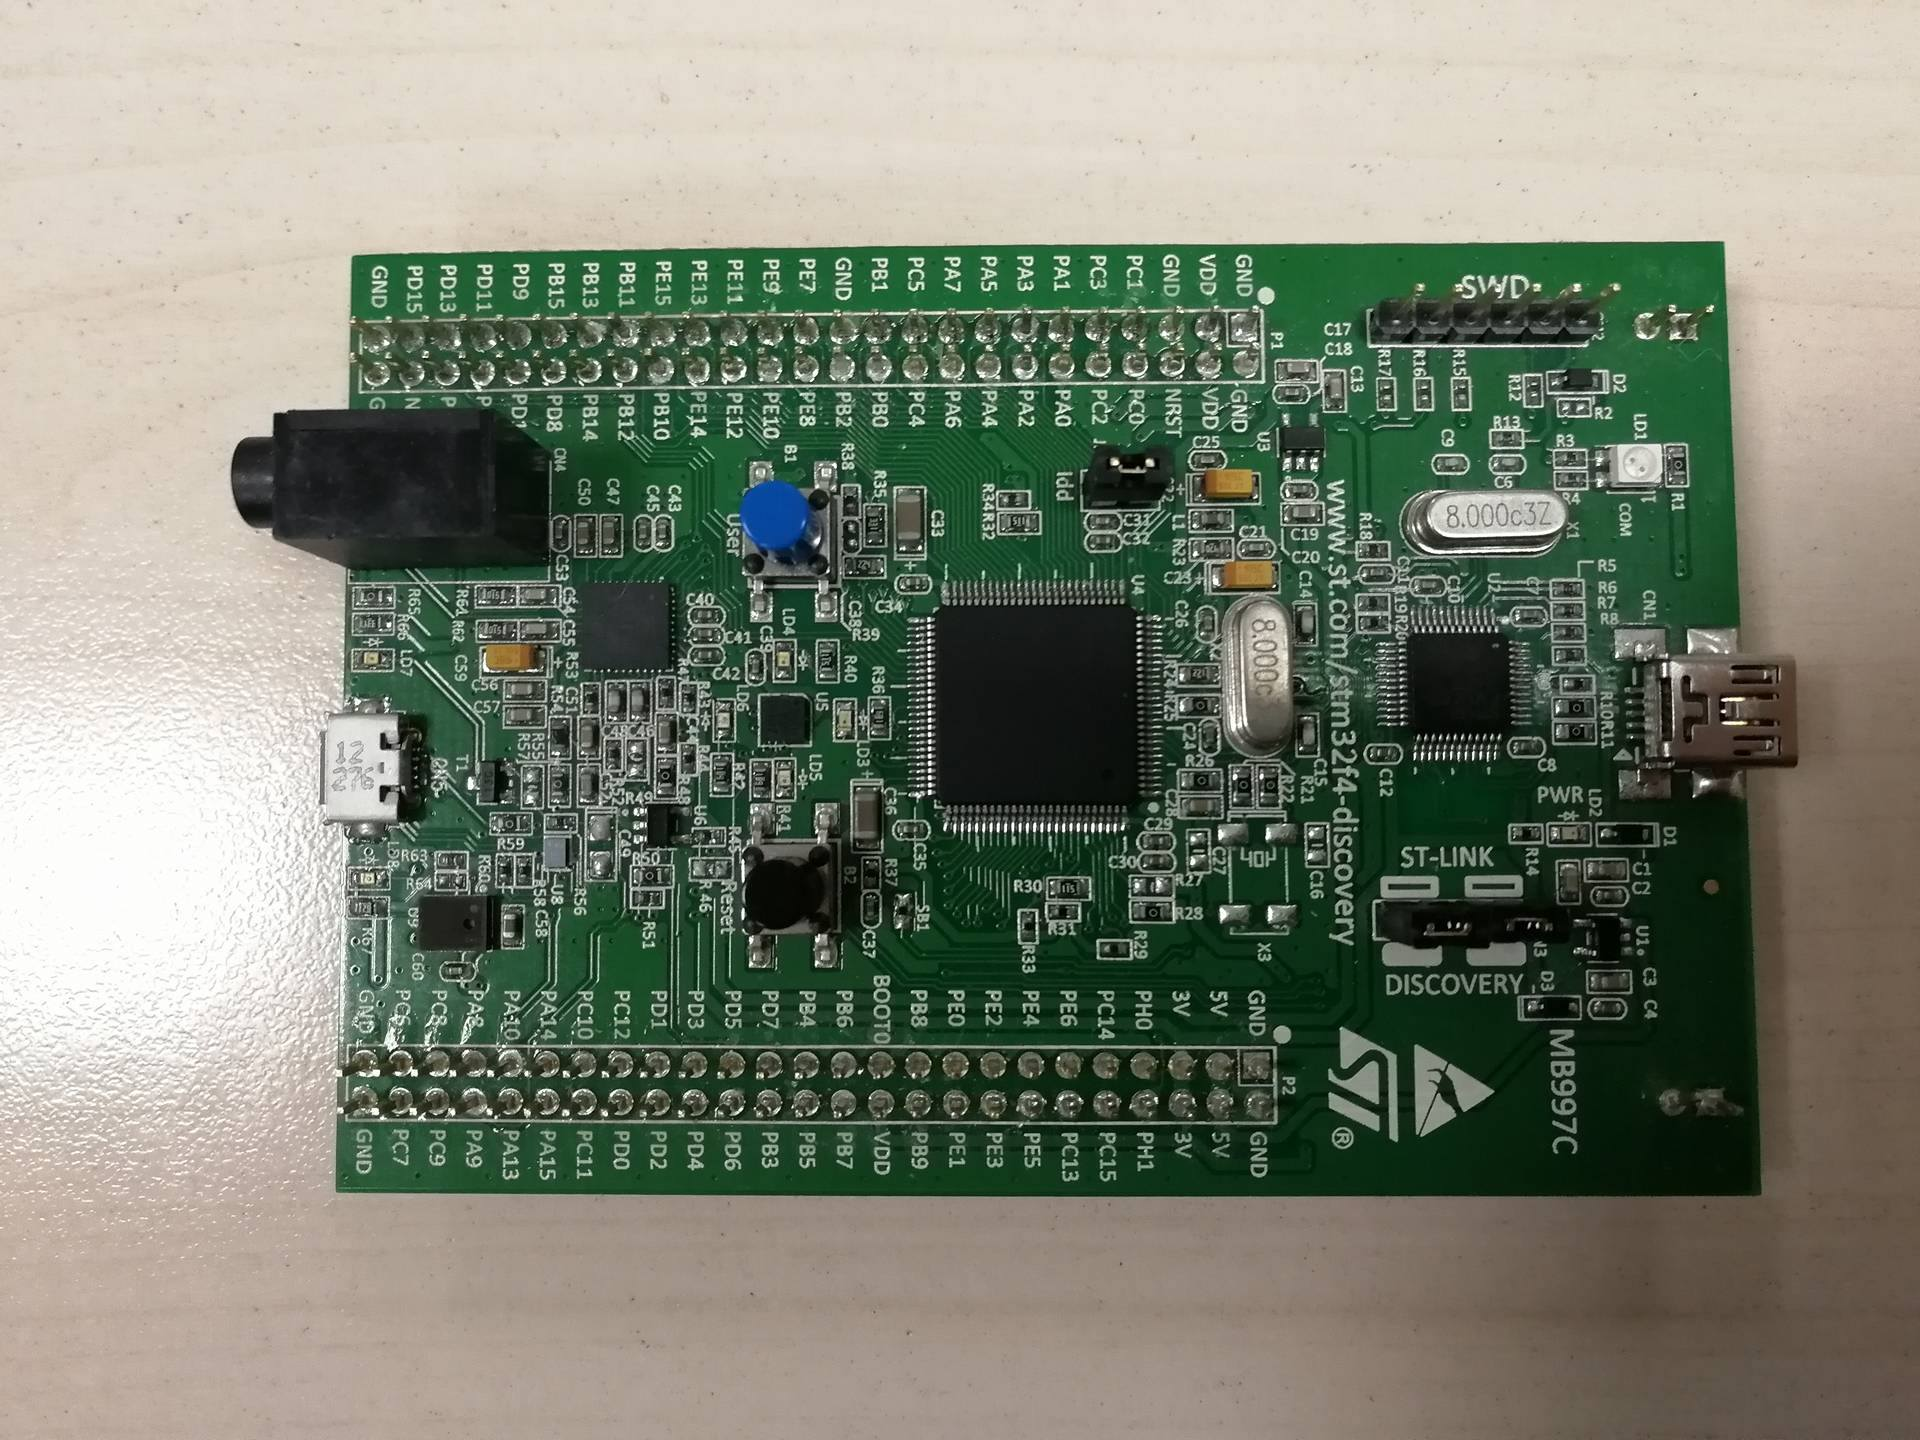
\includegraphics[width=0.7\textwidth]{./figures/board.jpg}
  \caption{Discovery Board}
  \label{fig:Board}
\end{figure}

\begin{figure}[htbp]
  \centering
     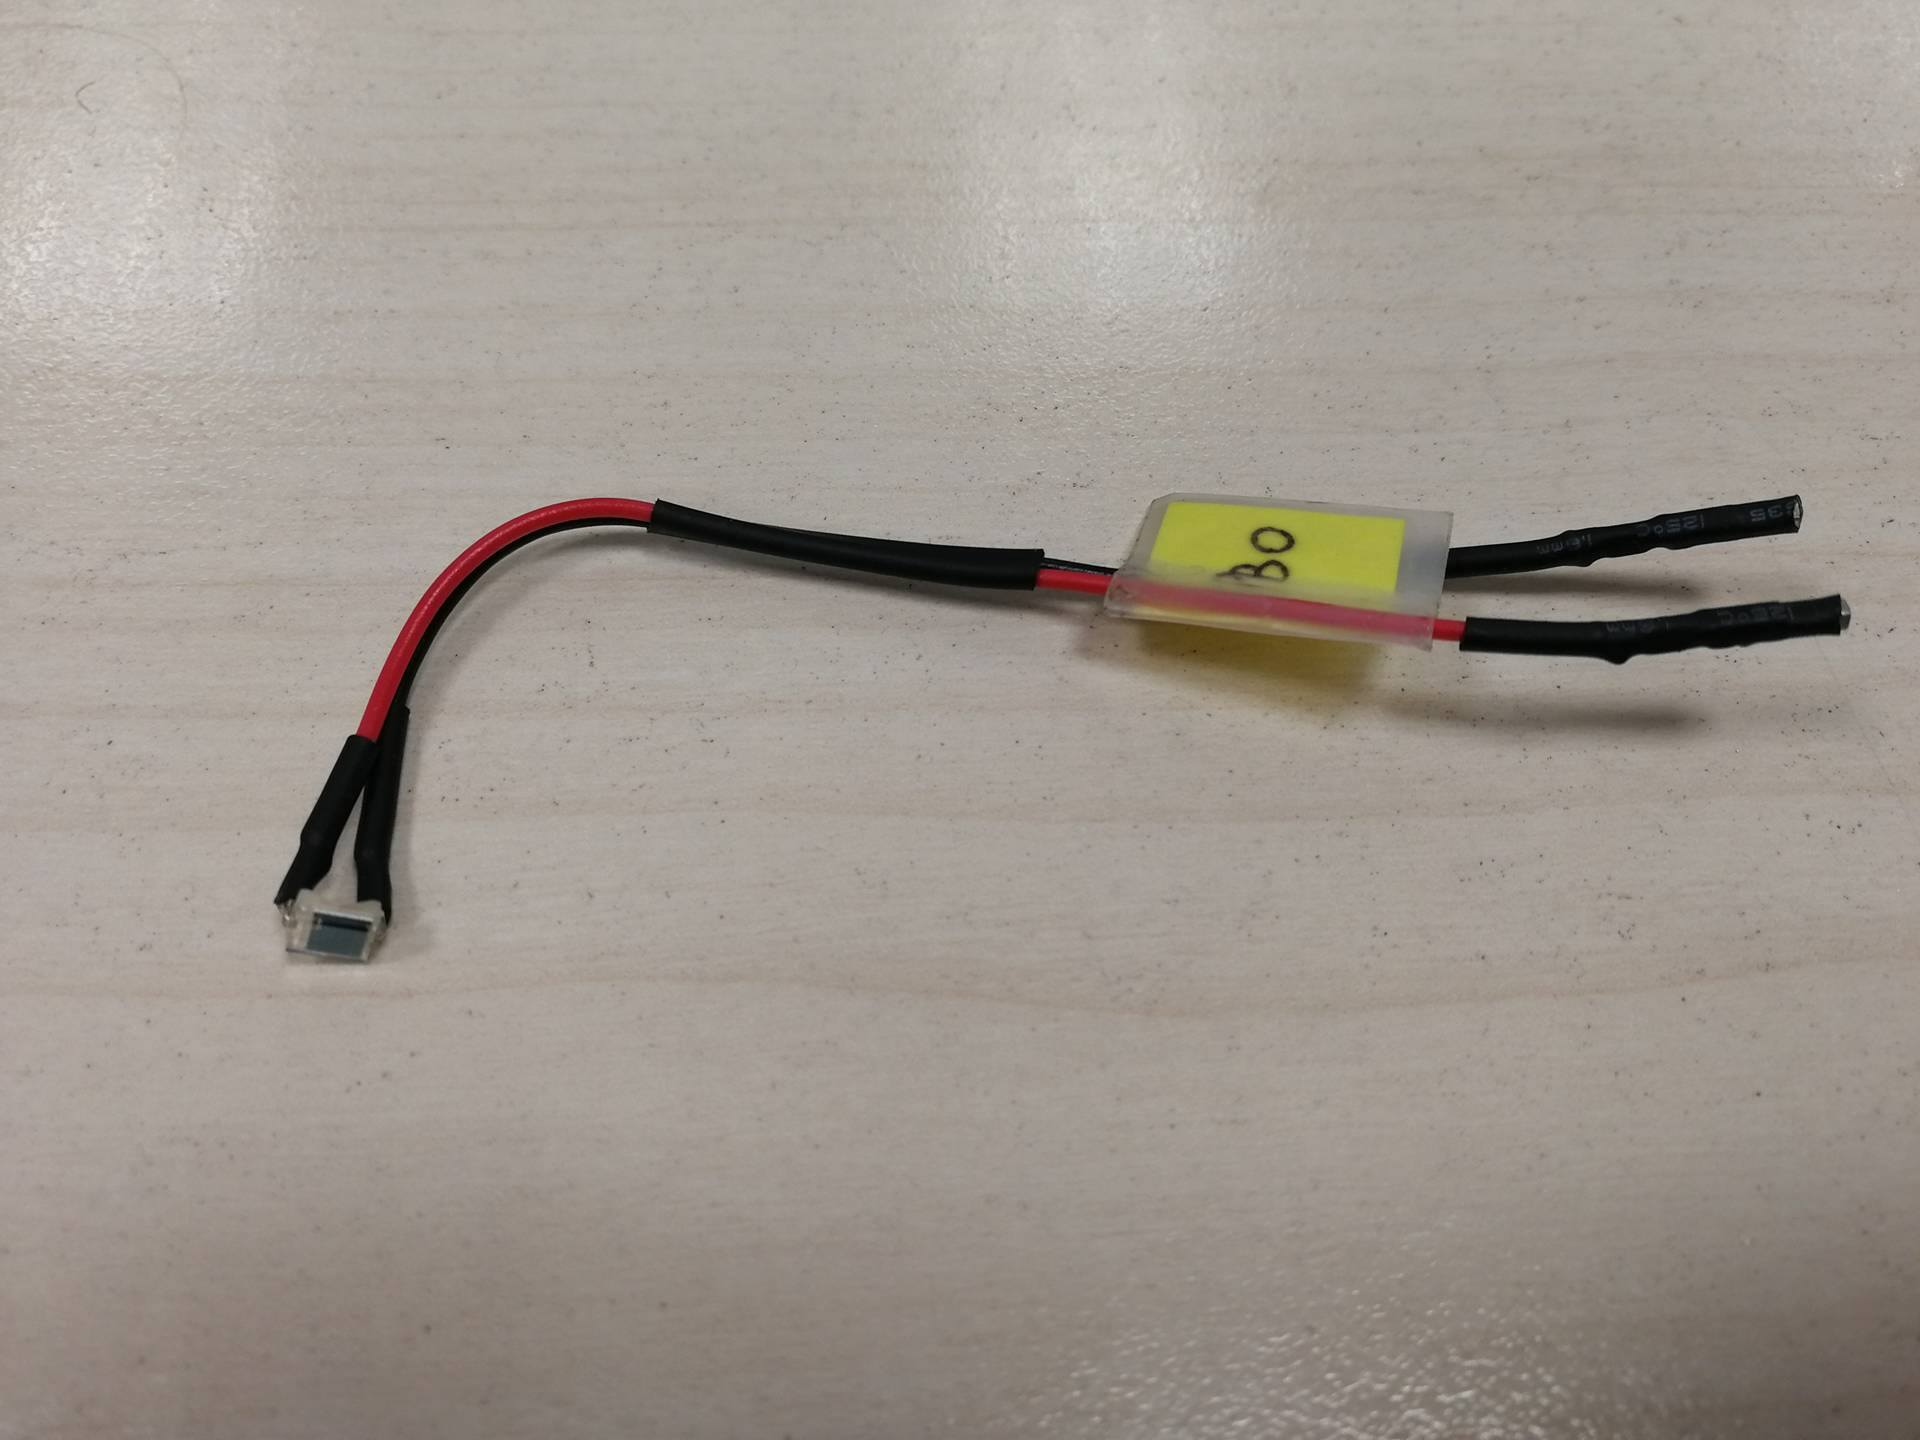
\includegraphics[width=0.5\textwidth]{./figures/photodiode.jpg}
  \caption{Photodiode}
  \label{fig:photodiode}
\end{figure}

\par
In this work the push buttons and LEDs were utilized that are located on the board. An external photodiode shown in figure \ref{fig:photodiode} was connected to the development board connection pins. The photodiode and the components mentioned above were used to make a simple game that measures the users reaction time.

\pagebreak


\section{Design and implementation}
\subsection{Game logic}
The idea of the implemented game was to test the reaction time of a player. This game can be played by a defined number of players. The reaction time of a player is evaluated by indicating a start signal and after this signal the player has to cover the photodiode as fast as possible to indicate a stop signal. The game logic is illustrated in figure \ref{fig:GameLogicDiagram}. 

\begin{figure}[htbp]
  \centering
     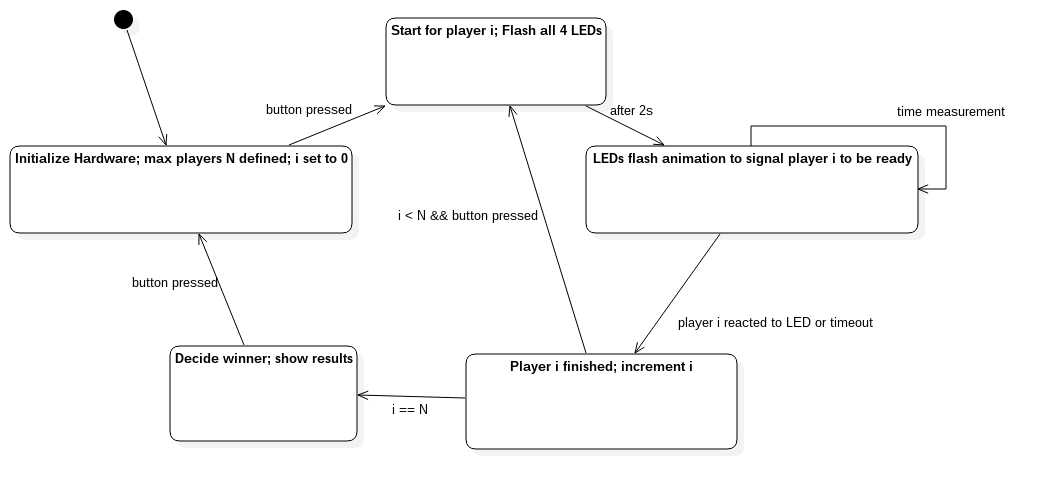
\includegraphics[width=1\textwidth]{./figures/FSM_Diagram.png}
  \caption{Game logic diagram}
  \label{fig:GameLogicDiagram}
\end{figure}

As illustrated in figure \ref{fig:GameLogicDiagram} the game is started after the hardware initialization has been completed. The game is started when the power of the board is turned on and the board's user push button has been pressed. Information about the game status and corresponding instructions are printed on a serial monitor. These instructions are shown in chapter \ref{Results}.\\
\par
After the push button has been pressed it is the first player's turn and all of the user programmable LEDs start to flash rapidly for a short duration and then the LEDs turn off. This is an indication to the player to get ready and be prepared to cover the photodiode soon. After this the LEDs start to light up in a clockwise orientation one by one. Once the fourth LED has lighten up, the player has to cover the photodiode as quickly as possible. Player reaction time is measured from the fourth LED lighting up and to the point when the photodiode has been covered.\\ 
\par
Then another player starts their turn by pressing the push button and has to interact with the system in the same manner as the player before. This cycle is repeated until all of the players have had their turn. The reaction times are finally displayed and the player who has had the lowest reaction time wins the game. A new game can be started by pressing the push button.

\subsection{Peripheral drivers}
For simplicity a design choice for this microcontroller project was to avoid the use of multiple threads. Every game logic procedure is executed in a sequential order and only interrupts allow to break this cycle and trigger events concurrently.\\
\par
In this project, interrupts are used by timers to toggle LEDs and for button detection. For the analog watchdog polling is utilized.
This approach allows to sense if the user tries to cheat by covering the photodiode before the fourth LED start to flash. As an alternative to this it would be also possible to realize the watchdog with interrupts and toggle the LEDs with sleep delays.\\
\par
The Miosix operating system (\cite{Miosix}) is included in the project workspace and is mainly used for a simplified accessing of the STM32F4 peripheral addresses by calling provided register names. Also the \emph{Timer} class for measuring time and the \emph{Random Number Generator} are exploited.

\subsubsection{ADC}
The control of the analog-to-digital converter builds the core of the project. A simple photodiode is connected to the board and the photodiode introduces an analog input voltage level depending on the ambient light intensity. The voltage has to be detected and read out as a digital signal in defined time intervals. Since the actual values are not important for this project, there is no data processing necessary. The values simply have to be compared to a threshold voltage and if they exceed this threshold, further action should be initiated. The analog watchdog provided by the microcontroller is used to execute this comparison.\\
\par
To enable the the analog-to-digital converter peripheral and to connect the general purpose input/ouptut (GPIO) pin to the ADC peripheral a set of registers were needed to be configured to enable this desired fucntionality. The desired implementation was to connect the light sensor to the first GPIO of port B (PB0) and connect that GPIO to the ADC.\\
\par
First the GPIO port where the light sensor was connected needs to be enabled. Since the light sensor was connected to PB0 pin, the port B clock must be enabled. This is achieved by setting the GPIOBEN bit in the RCC AHB1 peripheral clock enable register. In order to connect the GPIO to the ADC it was needed to configure the GPIO port to analog mode of the four possible operation modes. This was done by writing value of 11 to number of the pin number (0) in the GPIO port mode register.\\
\par
The ADC peripheral is setup after connecting the GPIO port to ADC. From the user manual of the development board \cite{UsrManual} the used GPIO could be conncected to first two ADC registers of the three available ADC registers of the microcontroller and connected to the input channel 8 of the ADC. It was decided to use the ADC1 of the microcontroller thus the corresponding clock was needed to be enabled from the RCC APB2 peripheral clock enable register.\\
\par
After setting up the GPIO register to be used in analog mode and connecting the register to the ADC the following functionality of the ADC was chosen:
\begin{itemize}
  \item Resolution: 12 bits
  \item Prescaler: PCLK2/8
  \item Sampling time of input channel (8): 84 cycles
  \item Data alignment: right data alignment
  \item Conversion mode: continuous conversion mode
\end{itemize}
All functionalities stated above could be set specifically for the ADC1 register except the prescaler value that was set in the common ADC register. Also the watchdog funcitonality of the ADC is utilized to see if the converted value is below a certain threshold that is calibrated everytime the ADC is initialized (board is powered on or reseted). The use of the watchdog functionality can be set specifically to be used in one of the three ADCs.

\subsubsection{Push button}
The user configurable push button (blue push button in figure \ref{fig:Board}) is used for starting a game after board setup, switching player turn and starting a new game. As stated before pressing the button causes an interrupt and signal the system that the button has been pressed. 
%TODO Arno


\subsubsection{LEDs \& Timer}
Since the toggling of the LEDs is realized with interrupts, the LED management explicitely includes a hardware timer. The \emph{Led} class knows three different operating modes: At the beginning of a game round all four LEDs flash rapidly, after that the number of blinking LEDs increase from 1 to 3 and finally after a random time interval also the fourth LED becomes active. For all these three modes only one timer (TIM3) needs to be utilized because the blinking procedures happen sequentially.\\
\par
For every sequence the function \emph{startLedTimer()} is called with a different time interval which sets the prescaler of the timer. Also the new LED mode is passed with the function. With the given mode every time the timer generates an overflow interrupt, the corresponding IRQ handler knows in which way the LEDs should be toggled.

\subsubsection{Serial}
%TODO Arno
The serial connection is utilized to display game instructions and the winner of the game in a terminal window of a machine. Communication with other devices is done by using the USART interface. The development board could be connected to a machine with a USB to TTL serial cable since the board itself doesn't a provide a way that the USART interface can communciate with USB. While using miosix the USART connections are predefined. The connection is made with pins PB10 and PB11 with PB10 being the transmitting side and PB11 being the receiving side. Also a operating voltage and ground was provided for the TTL cable. The messages sent by the microcontroller can be viewed with a terminal window application e.g. screen and using a correct baud rate indicated in the miosix source code. This value is 19200 
%black GND (not necessary?), yellow PB10, orange PB11
%sudo screen /dev/ttyUSB0 19200



\subsubsection{Connections}
The connections made are shown both in table 1 and figure 4 (CORRECT WITH REFS). 

\begin{figure}[htbp]
  \centering
     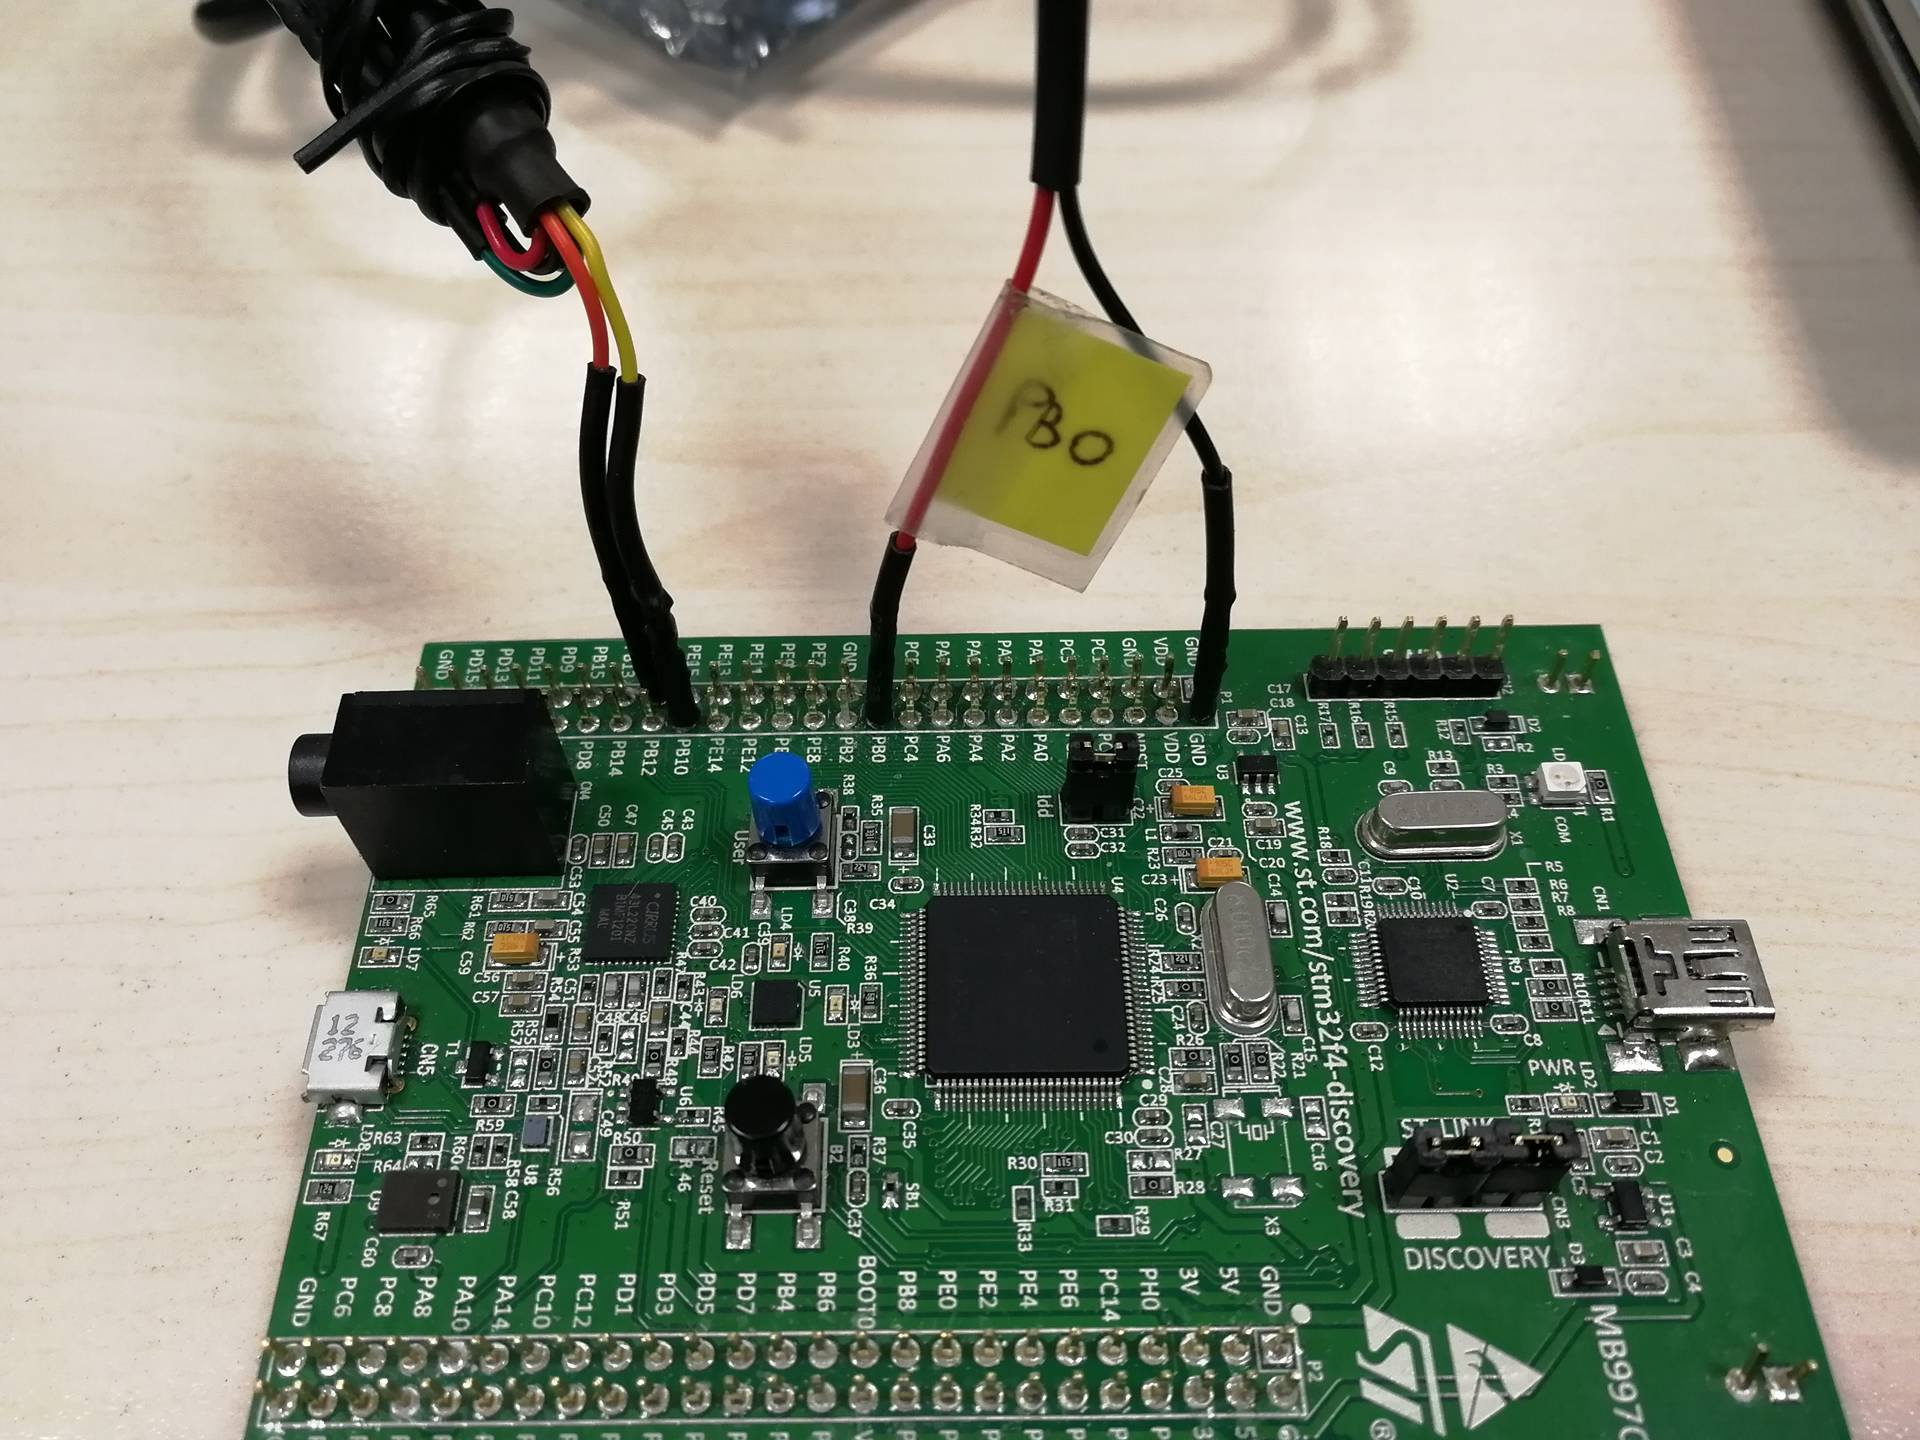
\includegraphics[width=1\textwidth]{./figures/connections.jpg}
  \caption{Connections}
  \label{fig:connections}
\end{figure}

\section{Results}
The operation of the system was tested multiple times in order to test the functionality of the system and also in different locations in order to test the analog watchdog threshold set correctness. After testing the system in different lcoations the system was operating similarly everytime and thus it was concluded that the system is working correctly. In the following is a sample run of the system:

\section{Conclusions}
This project was about implementing a analog-to-digital converter driver for the STM32f407 microcontroller and utilizing it with a light sensor. Also the STM32 F4 Discovery kit development board was utilized to prdouce a user reaction time game with using the boards LEDs and pusbutton.\\
\par
The most emphasis of this project was on implementing the ADC driver. The most challening part of constructing the driver was interfacing the used GPIO and ADC registers.
%TODO Arno
